\documentclass[../../main.tex]{subfiles}

\lstset{basicstyle=\small,
      showstringspaces=false,
      commentstyle=\color{black},
      keywordstyle=\color{blue}
    }
\emergencystretch 1em  % F"ur TeX <3.0 auskommentieren!
\graphicspath{{images/SignalErkennung/}{../../images/SignalErkennung/}}


\begin{document}

\subsection{Schild- und Numererkennung}
In diesem Kapitel wird die Schild- und Numererkennung des Soul- Trains erläutert. Die Schild- und Nummererkennung muss drei Aufgaben erfüllen:
\begin{itemize}
  \item Erkennung der Schilder (grosse- / kleine- Tafel)
  \item Erkennung der Nummer auf dem Schild
  \item Erkennung des Startsignals
\end{itemize}

Wie im Abbildung \ref{fig:ausschnitt_Anforderungsliste} ersichtlich, wurde im Rahmen des PREN 1 die Erfüllung der Funktionalität bei einer mindestgeschwindigkeit von 0.5 m/s als Anforderung vorausgesetzt. 

\begin{figure}[H] %Anforderungsliste
  \centering
  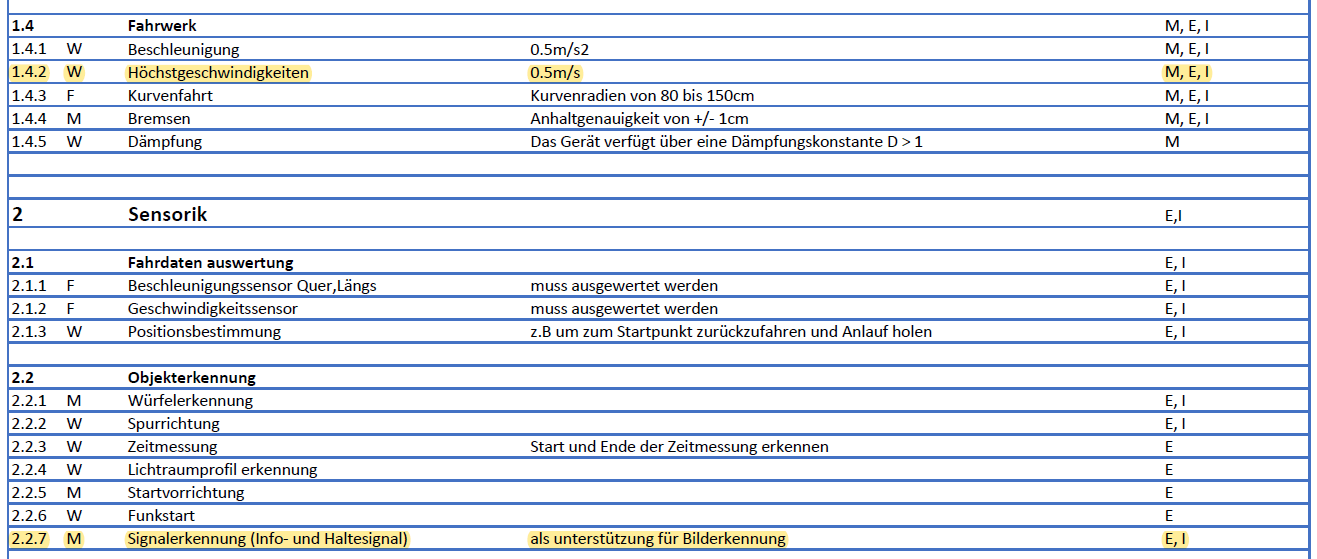
\includegraphics[width=1\textwidth]{Anforderung.png}
  \caption{Ausschnitt der Anforderungsliste PREN 1}
  \label{fig:ausschnitt_Anforderungsliste}
\end{figure}


\subsubsection{Hardware}
Für diese rechenintensiven Aufgaben wurde ein zusätzlicher Platinenrechner eingesetzt. Zum Einsatz kommt ein Raspberry PI 3 A+ [2]. Dieser verfügt wie sein «grosser Bruder» Raspberry PI 3 B+ [3] einen 64bit Cortex- A53 (ARMv8) SoC und einem 5GHz IEEE 802.11.ac Wireless LAN. Ihm stehen aber im Gegensatz zum B+ Model nur 512MB LPDDR2 RAM zur verfügung.   

\begin{figure}[H] %Antriebswagen mit RPI
  \centering
  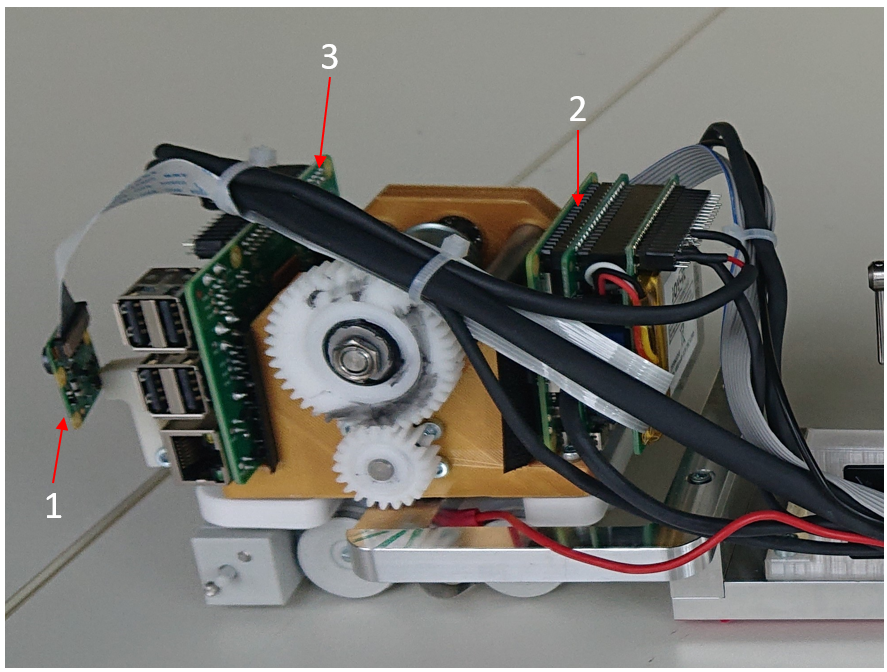
\includegraphics[width=0.5\textwidth]{RPI-uebersicht.png}
  \caption{Ausschnitt der Anforderungsliste PREN 1}
  \label{fig:rpi-uebersicht}
\end{figure}

In PREN 1 wurde ein Raspberry PI Zero W für diese Aufgabe vorgesehen. Dieser musste aber Aufgrund des schwachen Prozessors durch den 3 A+ ersetzt werden. Dank genügend vorhandenen Platz und des geringen Preisaufschlags konnte dieser wechsel problemlos durchgeführt werden. Dafür kann nun auch die Nummererkennung komplett auf diesem Platinenrechner durchgeführt werden. Als Kamera kommt wie in PREN 1 evaluiert die Standartkamera vom Raspberry PI [1] mit der CSI (Camera Serial Interface) zum Einsatz.

\subsubsection{Software: Ablaufsteuerung}
Als Basisarchitektur des Slave- RPI (Raspberry PI 3 A+) kommt eine «State- Machine» zum Einsatz. Angebunden ist diese an der übergeordneten Middleware, welche die Verbindung zum Master- RPI (Raspberry PI 3 B+) sicherstellt. Mehr dazu im Kapitel TODO: Kaptielreferenz zur Middleware. Der Ablauf, welcher den Slave- RPI tangiert, ist unterteilt in Phasen wie in Tabelle \ref{tab:Phasentabelle} ersichtlich.

\begin{table}[H] % Tabelle mit Phasen
  \begin{flushleft}
      \begin{tabular}{ | p{3cm} | p{10.5cm} |}
          \hline
          \textbf{Phase}  & \textbf{Beschreibung} \\\hline
          Startbereich & Erkennung des Startsignals \\\hline
          Runde 1      & Erkennung der grossen Tafel \& Nummererkennung \&  Erkennung des Startsignals \\\hline
          Runde 2      & Erkennung der grossen Tafel \& Nummererkennung \& Erkennung des Stopsignals \\\hline
          Runde 3      & Erkennung der kleinen Tafel \\\hline
      \end{tabular}
  \end{flushleft}
  \caption{Darstellung der Phasen für Slave- RPI}
  \label{tab:Phasentabelle}
\end{table}

Daraus lässt sich die State- Machine wie in Abbildung \ref{fig:state-machine} ableiten.
\vspace{1cm}

\begin{figure}[H] %State- Machine
  \centering
  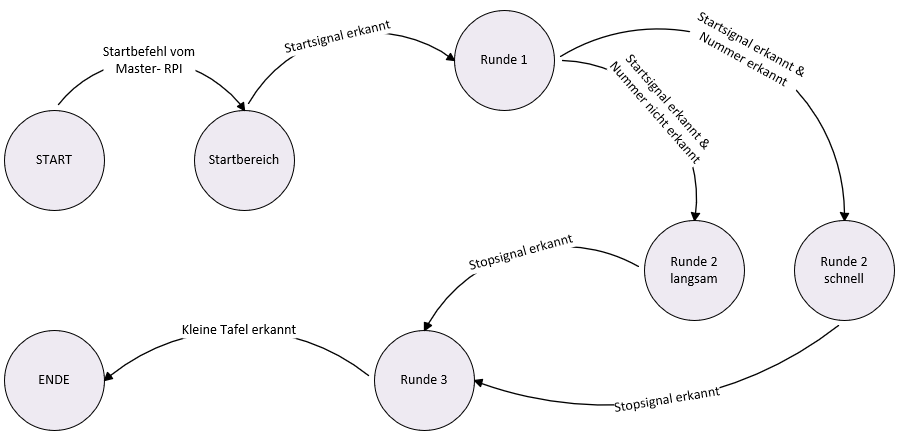
\includegraphics[width=0.9\textwidth]{state-machine.png}
  \caption{State- Machine Slave- RPI}
  \label{fig:state-machine}
\end{figure}

\newpage

\textbf{State: START}\\
Im Zustand \textit{START} wartet der Slave- RPI bis vom Master- RPI der Befehl «Start» via Middleware gesendet wird. Dieser Befehl wird vom Master- RPI nach dem erfolgreichen Würfelaufnahme dem Slave- RPI gesendet. Anschliessend wechselt der Slave- RPI zum Zustand \textit{Startbereich}\\

\textbf{State: Startbereich}\\
Im Zustand \textit{Startbereich} versucht der Slave- RPI das Startsignal (blau) zu erkennen. Dabei fährt der Zug im normalen Tempo. Sobald das Startsignal erkannt wird sendet der Slave- RPI via Middleware dem Master- RPI den Befehl \textbf{«11»} für die erste Runde. Anschliessend wechselt der Slave- RPI zum Zustand \textit{Runde1}.\\

\textbf{State: Runde 1}\\
Im Zustand \textit{Runde 1} wird nun im normalen Tempo versucht die grosse Tafel mit der Nummer zu erkennen. Wird die Tafel und die Nummer erkannt und die Runde abgeschlossen (d.h. Startsignal wurde auch erkannt), wechselt der Slave- RPI zum Zustand \textit{Runde 2 schnell}. Wird aber die Tafel oder die Nummer nicht erkannt und die Runde wird abgeschlossen, wechselt der Slave- RPI in den Zustand \textit{Runde 2 langsam}.\\

\textbf{State: Runde 2 schnell}\\
Im Zustand \textit{Runde 2 schnell} wird nun nicht mehr auf die grossen Tafeln und Nummern geachtet. Dem Master- RPI wird der Befehl \textbf{«22»} gesendet. Mit dem Befehl \textbf{«22»} an den Master- RPI, weiss dieser nun er kann mit vollem Tempo fahren. In der Runde 2 wird nur noch auf das Stopsignal geschaut, damit der Slave- RPI in den Zustand \textit{Runde 3} wechseln kann.\\

\textbf{State: Runde 2 langsam}\\
Im Zustand \textit{Runde 2 langsam} wird nochmals in der 2. Runde versucht die grosse Tafel mit der Nummer zu erkennen. Der Zug fährt weiterhin mit gleichem Tempo wie in der Runde 1 weiter. Gleichzeitig wird auf das Stopsignal für den wechsel in den Zustand \textit{Runde 3} geschaut.\\

\textbf{State: Runde 3}\\
Im Zustand \textit{Runde 3} wird dem Master- RPI der Befehl \textbf{«31»} gesendet. Nun wird das Tempo des Zuges auf ein minimum verzögert, damit das Anhalten so genau wie möglich erfolgen kann. Dabei versucht der Slave- RPI die kleine Tafel mit der Nummer zu erkennen. Sobald diese erkannt wird, wechselt der Slave- RPI in den Zustand \textit{ENDE}.\\

\textbf{State: ENDE}\\
Im Zustand \textit{ENDE} wird dem Master- RPI der Befehl \textbf{«0»} gesendet. Nun wird der Zug gestopt und das Programm des Slave- RPI ist abgeschlossen.

\newpage

\subsubsection{Software: Tafel- und Nummererkennung}
Im PREN1 konnte schon viele Versuche im Bereich der Tafel- und Nummererkennung durchgeführt werden. Die daraus resultierenden Erkenntnisse konnten im PREN 2 gut verwendet werden. Im folgenden werden die einzelnen Aufgaben (Tafel-, Start/ Stop- und Nummererkennung) einzeln behandelt und erläutert. \\

\textbf{Start-/ Stop- Signalerkennung}\\
Das Start- / Stop- Signal (im weiteren nur noch Startsignal genannt) befindet sich nach dem Startbereich und signalisiert den jeweiligen Start der nächsten Runde. Das Signal besteht wie in Abbildung \ref{fig:startsignal} aus zwei blauen Rechtecken auf weissem Hintergrund. 

\begin{wrapfigure}{r}{0.4\textwidth} %Startsignal
  \begin{center}
    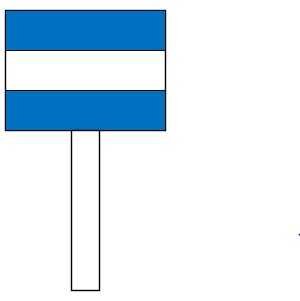
\includegraphics[width=0.3\textwidth]{startsignal.png}
  \end{center}
  \caption{Startsignal}
  \label{fig:startsignal}
\end{wrapfigure}

Um das Signal zu erkennen wird dafür das Bildverarbeitungsframework OpenCV verwendet. Das Startsignal verfügt mit den blauen Streifen über ein Alleinstellungsmerkmal. Dies wird für die Erkennung ausgenützt. Mittels \textbf{HSV- Filter} kann auf den genauen Farbraum gefiltert werden. So kann die Farbe Blau extrahiert werden. Als zweiter Schritt wird anschliessend Konturen erfasst und auf bestimmte Form und Grösse gefiltert. Da zwei blaue Streifen vorhanden sind, sollten jeweils zwei Treffer vorhanden sein. Wenn dies zutrifft wurde das Startsignal erkannt. Im Abbildung \ref{fig:codesnipped_startfilter} links ist die Filterfunktion mit HSV- und Konturfilter ersichtlich.

\vspace{0.5cm}

\begin{figure}[H] %Codesnipped Startsignalfilter
  \centering
  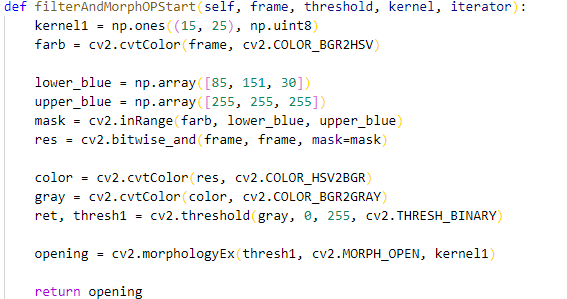
\includegraphics[width=0.7\textwidth]{codesnipped-filterStart.png}
  \caption{Codesnipped: Filter Startsignal}
  \label{fig:codesnipped_startfilter}
\end{figure}

\vspace{1cm}

\begin{table}[H] % Tabelle mit Phasen
  \begin{flushleft}
      \begin{tabular}{ | p{3cm} | p{10.5cm} |}
          \hline
          \textbf{Filter}  & \textbf{Beschreibung} \\\hline
          HSV          & Extraktion des blauen Farbraumes \\\hline
          Konturen     & Auf Grösse und Form der Konturen filtern\\\hline
      \end{tabular}
  \end{flushleft}
  \caption{Filter für Startsignalerkennung}
  \label{tab:filter_startsignal}
\end{table}

\newpage

\textbf{Tafelerkennung}\\
Die Tafel kann in zwei Ausführungen vorkommen. Weisse Zahl mit schwarzem Hintergrund oder umgekehrt. Für das Erkennen der Tafel kommen andere Filter wie beim Startsignalerkennung zum Einsatz. Anstatt einem HSV- Filter kommt bei der Tafelerkennung eine kombination von drei Filtern zum Einsatz. Als erstes kommt ein \textbf{Blur- Filter} zum Einsatz. Dieser sorgt dafür, dass alle «harten» Kanten im Bild \textit{weichgezeichnet} werden und somit können störeinflüsse reduziert werden. Anschliessend kommt die kombination \textbf{Binary- / OTSU- Filter} zum Einsatz. Diese Kombination dient dazu das Bild in ein \textit{Binary-Picture} zu transformieren und somit die Konturen zu extrahieren. Dabei wird ähnlich wie beim Startsignal die Konturen auf Grösse und Form gefiltert. 

\vspace{0.5cm}

\begin{figure}[H] %Tafelerkennung
  \centering
  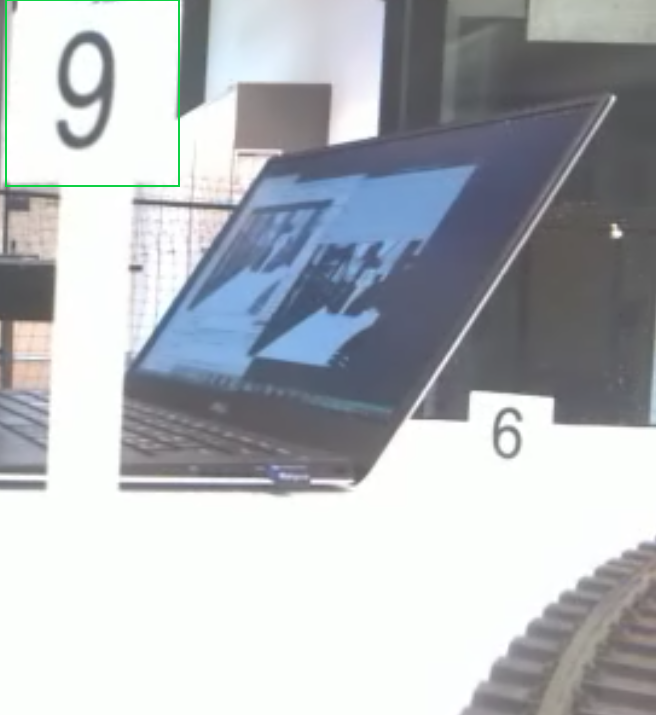
\includegraphics[width=0.4\textwidth]{tafel-weiss.png}
  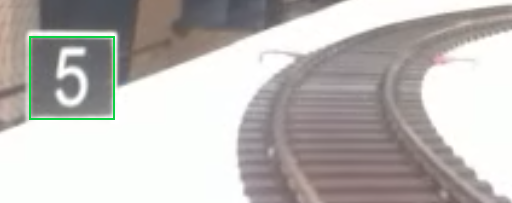
\includegraphics[width=0.4\textwidth]{tafel-schwarz.png}
  \caption{Tafelerkennung}
  \label{fig:tafelerkennung}
\end{figure}

\vspace{0.5cm}

\textbf{Nummerkennung}\\
Um nun die Nummer zu erkennen, wird ein Machine- Learning Framework eingesetzt. Erste Versuche im PREN 1 wurde mit der Bibliothek Keras und Backend Tensorflow durchgeführt. Für die Finale Version wurde aber auf die Software \textit{Tesseract OCR} von Google gesetzt, dies aus den Gründen der Effizienz. Tesseract OCR verfügt über einen Python Wrapper welcher einfach über den Packetinstaller \textit{pip} installiert werden kann. Tesseract selber kann einfach Mittels Sourcefiles kompiliert und installiert werden. In Abbildung ist ein Codesnipped für den TesseractWorker abgebildet. Ein grosser Vorteil von Tesseract OCR ist auch die Einfachheit. Nachdem die Konfigurationen gesetzt sind kann mittels einem Funktionsaufruf die erkannte Nummer zurückgegeben werden.

\begin{figure}[H] %Tesseract Codesnipped
  \centering
  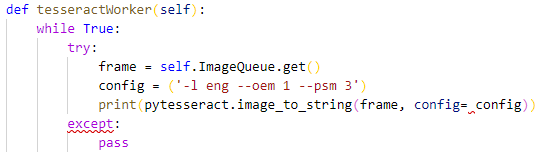
\includegraphics[width=0.8\textwidth]{codesnipped-tesseract.png}
  \caption{Codesnipped Tesseract}
  \label{fig:codesnipped_tesseract}
\end{figure}

\newpage

\textbf{Worker- Ablauf}\\


\end{document}